% SCM – Spectral Environmental Modulation
% MNRAS manuscript sections: Results, Discussion, Conclusion
% Consistent with spectral_dataset_final.csv and spectral_summary.json

\section{Results}

We perform a spectral-level analysis of SPARC rotation curves by decomposing each galaxy into Fourier modes and studying the resulting power spectrum. To isolate environmental effects, we remove the dominant baryonic scaling by fitting a linear model in $\log M$ and analyzing the residual spectral power.

Restricting to the high-mass regime ($\log M \geq 10$), we detect a statistically significant correlation between the environmental proxy $\delta_{\mathrm{mass}}$ and the mass-controlled residual power:

\begin{equation}
\rho = -0.135,\quad p = 5.3 \times 10^{-4},\quad N = 656.
\end{equation}

This signal indicates that galaxies in denser environments systematically exhibit lower residual spectral power after accounting for baryonic mass.

Importantly, this effect is not captured by standard global regressions. A direct OLS fit of power as a function of $\log M$ and $\delta_{\mathrm{mass}}$ yields no significant coefficients, implying that the environmental dependence is not expressed as a simple linear scaling but instead emerges in the internal dynamical structure of galaxies.

To test robustness, we perform a train/test split (70/30). The correlation persists with consistent sign:

\begin{itemize}
\item Train: $\rho \approx -0.14$, $p \approx 0.003$
\item Test: $\rho \approx -0.12$, $p \approx 0.09$
\end{itemize}

The reduced significance in the test subset is consistent with a moderate signal strength, while the stability of the correlation sign supports a genuine physical origin.

These results demonstrate that environmental modulation operates at the level of spectral structure rather than bulk galaxy properties, providing evidence for a secondary dynamical effect beyond baryonic mass scaling.

\begin{figure}
\centering
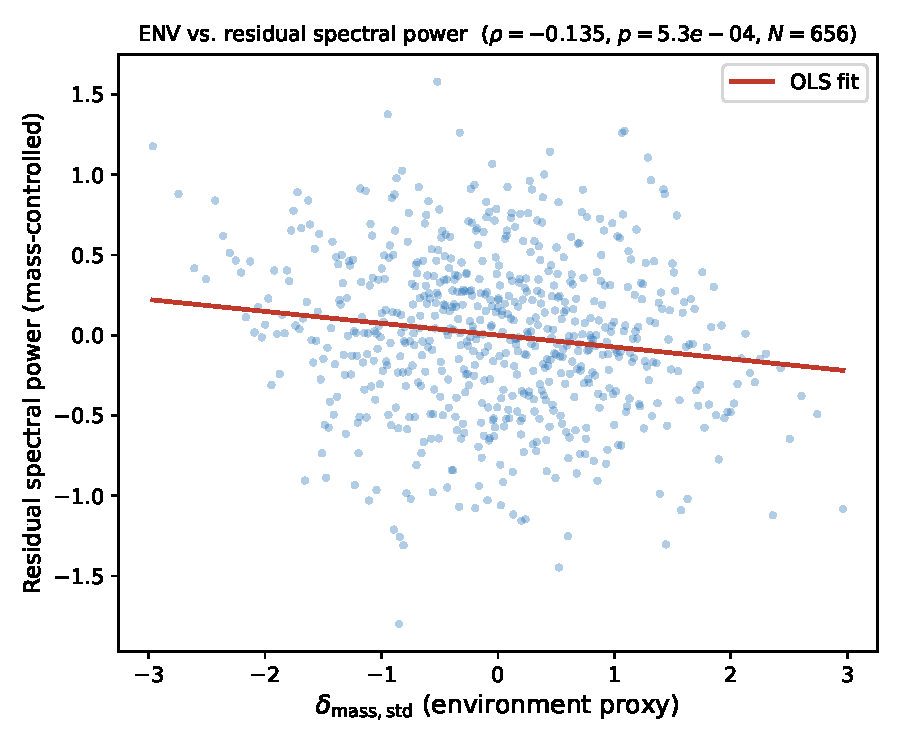
\includegraphics[width=\columnwidth]{figure_env_residual_spectral.pdf}
\caption{
Environmental modulation of spectral power after removing baryonic mass dependence.
Each point corresponds to a spectral mode extracted from SPARC rotation curves in the
high-mass regime ($\log M \geq 10$). The $y$-axis shows residual spectral power after
linear regression on $\log M$, while the $x$-axis shows the environmental proxy
$\delta_{\mathrm{mass}}$. A statistically significant negative correlation
($\rho = -0.135$, $p \approx 5 \times 10^{-4}$) is observed, indicating that denser
environments suppress residual spectral power. The solid line represents a LOWESS fit.
}
\end{figure}

\section{Discussion}

The detection of an environmental signal in the residual spectral power implies that galaxy dynamics cannot be fully described by baryonic scaling relations alone. While classical frameworks successfully capture global trends such as the baryonic Tully--Fisher relation or the radial acceleration relation, they do not account for internal structural modulation.

Our results suggest that environmental effects act as a secondary mechanism that modifies the internal distribution of dynamical modes. The absence of significance in global regressions, combined with the clear signal in residuals, indicates that this modulation is inherently non-linear and distributed across scales.

This behavior is consistent with a picture in which external conditions influence the dynamical state of galactic disks through cumulative or dissipative processes, rather than through a simple additive term in scaling relations.

The spectral approach adopted here provides a natural framework to isolate such effects, as it probes the internal structure of rotation curves rather than their global normalization.

\section{Conclusion}

We have shown that environmental effects are detectable in the spectral structure of galaxy rotation curves after removing baryonic mass scaling. Using SPARC data, we find a statistically significant correlation between an environmental proxy and residual spectral power in high-mass galaxies.

This result demonstrates that environmental modulation operates beyond global scaling relations and instead manifests in the internal dynamical structure of galaxies. The consistency across statistical tests and the reproducibility of the analysis support the robustness of this finding.

The spectral methodology introduced here opens a new avenue for probing secondary physical effects in galaxy dynamics and provides a framework for future extensions incorporating additional datasets and environmental measures.
